\documentclass[12 pt]{article}
\usepackage[utf8]{inputenc}
\usepackage{a4}
\usepackage{indentfirst}
\usepackage{graphicx}
\usepackage{float}
\usepackage{tabularx}
\usepackage{multicol}
\usepackage{tikz, adjustbox}
\usepackage[most]{tcolorbox}
\usepackage{wrapfig}
\usepackage{amssymb}
\usepackage{amsmath}
\usepackage{hyperref}
\newcolumntype{M}[1]{>{\centering\arraybackslash}m{#1}}
\usepackage{titlesec}
\usepackage{listings}
\usepackage{esint}
\usepackage{xcolor}
\usepackage{empheq} 
\setlength\parindent{0pt}
\definecolor{codegreen}{rgb}{0,0.6,0}
\definecolor{codegray}{rgb}{0.5,0.5,0.5}
\definecolor{codepurple}{rgb}{0.58,0,0.82}
\definecolor{backcolour}{rgb}{0.95,0.95,0.92}
\emergencystretch=1em
\lstdefinestyle{mystyle}{
    backgroundcolor=\color{backcolour},  
    commentstyle=\color{codegreen},
    keywordstyle=\color{magenta},
    numberstyle=\tiny\color{codegray},
    stringstyle=\color{codepurple},
    basicstyle=\footnotesize\ttfamily,
    breakatwhitespace=false,         
    breaklines=true,                 
    captionpos=b,                    
    keepspaces=true,                 
    numbers=left,                    
    numbersep=5pt,                  
    showspaces=false,                
    showstringspaces=false,
    showtabs=false,                  
    tabsize=2,
    frame=single,
}
\lstset{style=mystyle}
% Yellow:
\definecolor{BgYellow}{HTML}{FFF59C}
\definecolor{FrameYellow}{HTML}{F7A600}
% Pink:
\definecolor{BgPink}{HTML}{EF6FA7}
\definecolor{FramePink}{HTML}{E5446E}


% Yellow Sticky Note (YStkyNote):
\newtcolorbox{YStkyNote}[1][]{%
    enhanced,
    before skip=2mm,after skip=2mm, 
    width=0.6\textwidth, % width of the sticky note
    boxrule=0.2mm,
    colback=BgYellow, colframe=FrameYellow, % Colors
    attach boxed title to top left={xshift=0cm,yshift*=0mm-\tcboxedtitleheight},
    varwidth boxed title*=-3cm,
    % The titlebox:
    boxed title style={frame code={%
        \path[left color=FrameYellow,right color=FrameYellow,
        middle color=FrameYellow]
        ([xshift=-0mm]frame.north west) -- ([xshift=0mm]frame.north east)
        [rounded corners=0mm]-- ([xshift=0mm,yshift=0mm]frame.north east)
        -- (frame.south east) -- (frame.south west)
        -- ([xshift=0mm,yshift=0mm]frame.north west)
        [sharp corners]-- cycle;
        },interior engine=empty,
    },
    sharp corners,rounded corners=southeast,arc is angular,arc=3mm,
    % The "folded paper" in the bottom right corner:
    underlay={%
        \path[fill=BgYellow!80!black] ([yshift=3mm]interior.south east)--++(-0.4,-0.1)--++(0.1,-0.2);
        \path[draw=FrameYellow,shorten <=-0.05mm,shorten >=-0.05mm,color=FrameYellow] ([yshift=3mm]interior.south east)--++(-0.4,-0.1)--++(0.1,-0.2);
        },
    drop fuzzy shadow, % Shadow
    fonttitle=\bfseries, 
    title={#1}
}
% Pink Sticky Note (PStkyNote):
\newtcolorbox{PStkyNote}[1][]{%
    enhanced,
    before skip=2mm,after skip=2mm, 
    width=0.4\textwidth, % width of the sticky note
    boxrule=0.2mm, 
    colback=BgPink, colframe=FramePink, % Colors
    attach boxed title to top left={xshift=0cm,yshift*=0mm-\tcboxedtitleheight},
    varwidth boxed title*=-3cm,
    % The titlebox:
    boxed title style={frame code={%
        \path[left color=FramePink,right color=FramePink,
        middle color=FramePink]
        ([xshift=-0mm]frame.north west) -- ([xshift=0mm]frame.north east)
        [rounded corners=0mm]-- ([xshift=0mm,yshift=0mm]frame.north east)
        -- (frame.south east) -- (frame.south west)
        -- ([xshift=0mm,yshift=0mm]frame.north west)
        [sharp corners]-- cycle;
        },interior engine=empty,
    },
    sharp corners,rounded corners=southeast,arc is angular,arc=3mm,
    % The "folded paper" in the bottom right corner:
    underlay={%
        \path[fill=BgPink!80!black] ([yshift=3mm]interior.south east)--++(-0.4,-0.1)--++(0.1,-0.2);
        \path[draw=FramePink,shorten <=-0.05mm,shorten >=-0.05mm,color=FramePink] ([yshift=3mm]interior.south east)--++(-0.4,-0.1)--++(0.1,-0.2);
        },
    drop fuzzy shadow, % Shadow
    fonttitle=\bfseries, 
    title={#1}
}

\title{\huge{Lecture Notes 2: Basic laws of static electricity}}
\author{}
\date{}
\begin{document}
\maketitle
\tableofcontents
\newpage
\section{Coulomb's law}
It's an experimental law of physics that measures the force between two stationary, electrically charged particles.
\subsection{Observations}
\begin{minipage}{0.6\linewidth}
\begin{itemize}
    \item There's an attraction/repulsion force between electrically charged particles
    \item This force is $\propto \frac{Qq}{r^2}$
    \item The force is in the direction $\underline{u_r}$
    \item It's analogous to newton's law of gravitational force
\end{itemize}
\end{minipage}
\begin{minipage}{0.38\linewidth}
    \begin{figure}[H]
    \centering
    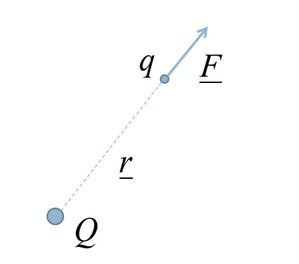
\includegraphics[scale=0.35]{./images/coul1}
    \caption{coulomb's law}
    \label{coul1} 
\end{figure}
\end{minipage}
\subsection{Mathematical Modeling}
$$\underline{F}=\frac{Qq}{4\pi \epsilon_{0} r^2}\quad \underline{u_r}$$
where $\epsilon_0$ is the permittivity in free space $\left(\frac{10^{-9}}{36\pi} F/m \right)$
\section{Electrostatic field intensity vector}
\begin{minipage}{0.59\linewidth}
Any electric charge has an electric field that surrounds it, and it depends on:\begin{itemize}
    \item distance from the charge
    \item the medium
    \item the intensity of electric charge
\end{itemize}
\end{minipage}
\begin{minipage}{0.4\linewidth}
    \begin{figure}[H]
    \centering
    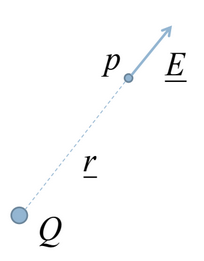
\includegraphics[scale=0.35]{./images/electrostatic1}
    \caption{Electrostatic field at p}
    \label{electro1} 
\end{figure}
\end{minipage}
\newpage
\subsection{Mathematical Modeling}
$$\underline{E_p}=\frac{Q}{4\pi \epsilon_{0} r^2}\; \underline{u_r} \;=\frac{\underline{F}}{q}$$
We assume that we are calculating the force acting on a charge (q) with magnitude equal to 1 at point p.
\subsubsection{Can electric field be equal to infinity?}
In the above equation if we placed $r=0$, then $E=\infty$, But actually "r" can never be 0, as when we get very close to a point charge, it acts as a spherical charge with radius "a" as shown in the figure below \ref{electro3}, and "a" can never be 0 
\begin{minipage}{0.45\linewidth}
    \begin{figure}[H]
    \centering
    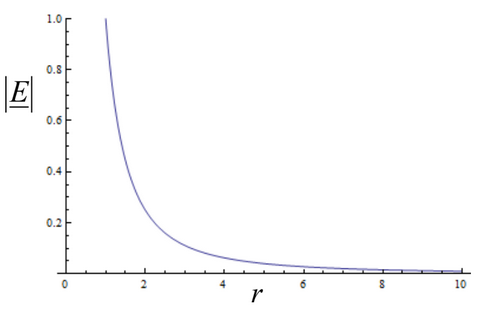
\includegraphics[scale=0.35]{./images/electrostatic2}
    \caption{E and r graph}
    \label{electro2} 
    \end{figure}
\end{minipage}
\begin{minipage}{0.5\linewidth}
    \begin{figure}[H]
    \centering
    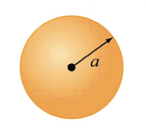
\includegraphics[scale=0.85]{./images/electrostatic3}
    \caption{spherical charge}
    \label{electro3} 
    \end{figure}
\end{minipage}
\section{Superposition of electrostatic field}
Every charge in space creates an electric field at point independent of the presence of other charges in that medium. The resultant electric field is a vector sum of the electric field due to individual charges.

\begin{minipage}{0.35\linewidth}
$$
\underline{E_p}=\sum_{i=1}^{N}\frac{q_i}{4\pi \epsilon_{0} r_i^2}\quad \underline{u_i}
$$
\end{minipage}
\begin{minipage}{0.6\linewidth}
    \begin{figure}[H]
        \centering
        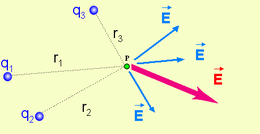
\includegraphics[scale=0.7]{./images/superposition1}
        \caption{superposition of electrostatic field}
        \label{super1} 
    \end{figure}
\end{minipage}
\newpage
\section{Electrostatic field of a continuum of charges}
Until this moment, we have been talking about point charges, so let's try to generalize what we have achieved, Let's consider a random 3D shape, as shown in the figure below \ref{cont1}. 
    \begin{figure}[H]
        \centering
        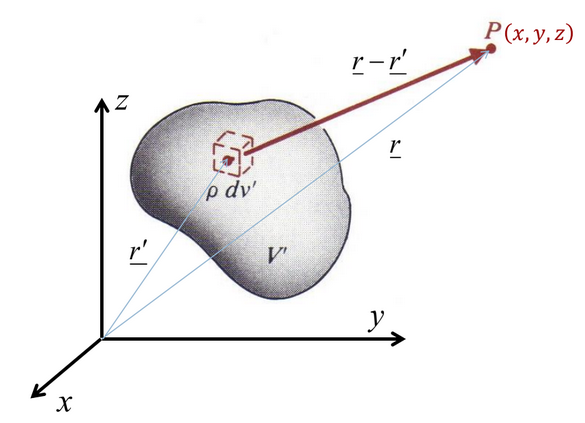
\includegraphics[scale=0.45]{./images/cont1}
        \caption{Random 3D shape of charges}
        \label{cont1} 
    \end{figure}
We can divide this shape into infinitesimal charge elements ($dq$) each charge element of them will be defined in terms of the volume it acquires($dq=\rho \, dv`$)
\subsection{Mathematical Modeling}
$$
E_p=\int_V \frac{dq}{4\pi\epsilon_0\left(\underline{r}-\underline{r`}\right)^2}\quad {u_{\underline{r}-\underline{r`}}} 
$$
$$\because u_{\underline{r}-\underline{r`}}=\frac{\underline{r}-\underline{r`}}{|\underline{r}-\underline{r`}|} \quad\quad \text{and}\quad\quad dq=\rho\, dv`$$

$$\boxed{\therefore E_p=\int_V \frac{\rho \, dv`}{4\pi\epsilon_0\left(\underline{r}-\underline{r`}\right)^3}\quad {\left(\underline{r}-\underline{r`}\right)}}$$
\newpage
\section{Electrostatic field lines}
They are visual representation of electric field, and they have the following properties: \begin{itemize}
    \item The direction of a field Line must be in the direction of the total field at the point.
    \item The lines depart from positive charges and terminate on negative charges.
    \item The lines are open and non-intersecting.
    \item The surface density of the lines crossing normally an element of surface area at a point in space gives the magnitude of the field at this point.
\end{itemize}
\subsection{visualization}
\begin{minipage}{0.5\linewidth}
    \begin{figure}[H]
    \centering
    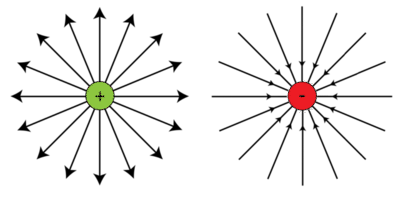
\includegraphics[scale=0.5]{./images/charges}
    \caption{point charges field lines}
    \label{charges} 
    \end{figure}
\end{minipage}
\begin{minipage}{0.45\linewidth}
    \begin{figure}[H]
    \centering
    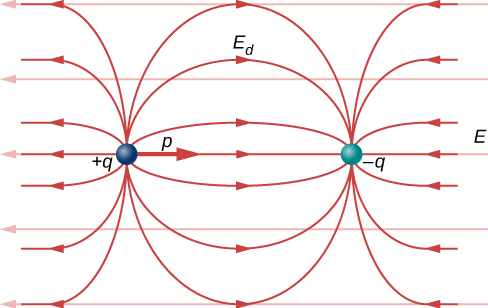
\includegraphics[scale=0.68]{./images/dipole}
    \caption{dipole field lines}
    \label{dipole} 
    \end{figure}
\end{minipage}
\section{Electrostatic flux }
\textbf{Electrostatic flux($\mathbf{\psi}$):} The number of field lines crossing normally an area of space in the field of electrostatic system of charges

\subsection{Mathematical modeling}
\begin{minipage}{0.35\linewidth}
$$
|\underline{E}|=\frac{d\psi}{ds_{\perp}}
$$
$$
d\psi=|\underline{E}| ds_{\perp}
$$
$$
\quad \quad \quad \quad=|\underline{E}| |\underline{ds}| cos(\alpha)
$$
$$
\quad = \underline{E} \cdot \underline{ds}
$$
$$
\boxed{\psi= \int_s \underline{E}.\underline{ds}}
$$
\end{minipage}
\begin{minipage}{0.6\linewidth}
    \begin{figure}[H]
        \centering
        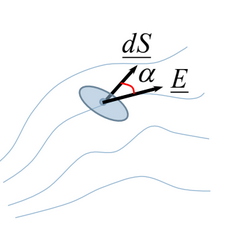
\includegraphics[scale=0.5]{./images/flux1}
        \label{flux1} 
    \end{figure}
\end{minipage}
\section{Electrostatic flux leaving a point charge}
How can you determine the electrostatic flux lines leaving a point charge? The idea is simple. If you put this point charge inside any closed surface -as shown in the figure below \ref{closed}- then you can use the mathematical equation we derived above to calculate the flux lines.
    \begin{figure}[H]
        \centering
        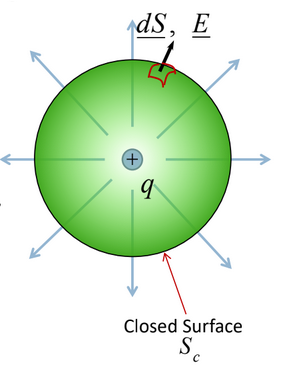
\includegraphics[scale=0.5]{./images/closed}
        \caption{Closed surface}
        \label{closed} 
    \end{figure}
\subsection{Why spherical coordinates}
As we said, you can put the point charge inside any closed surface, so why did we choose a sphere? It's because a point charge is like a tiny sphere, so the math will be a lot easier -as we are going to see- if we used spherical coordinates. Choosing cylindrical coordinates, or cartesian ones should still give the correct answer, however, the integration will just be difficult.
\subsection{Mathematical modeling}
$$
\psi =\oint_{s_c} \underline{E} \cdot \underline{ds}
$$
$$
\psi=\int_{0}^{\pi} \int_{0}^{2\pi} \frac{q}{4\pi\epsilon_0 r^2}\;\underline{ur}\cdot r^2 sin(\theta)\,d\theta d\phi\,\underline{u_r} 
$$
$$
\psi= \frac{q}{4\pi \epsilon_0}(2)(2\pi)
$$
$$
\boxed{
    \psi=\frac{q}{\epsilon}
}
$$
\section{Gauss's law for electrostatics field}
The total outward flux of the E-field over any closed surface in free space is equal to the total charge enclosed
by the surface divided by $\epsilon_0$
\subsection{Mathematical modeling}
\begin{minipage}{0.35\linewidth}
$$
\boxed{\psi= \oint_s \underline{E}.\underline{ds}=\frac{1}{\epsilon_0} \sum_{\text{inside }s_c}Q}
$$
\end{minipage}
\begin{minipage}{0.6\linewidth}
    \begin{figure}[H]
        \centering
        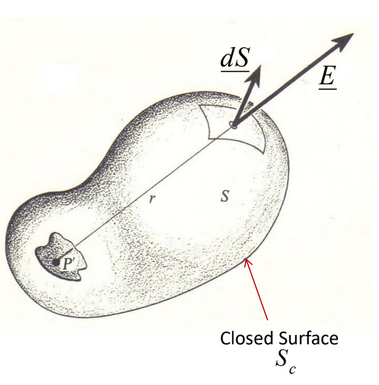
\includegraphics[scale=0.5]{./images/gauss}
        \label{gauss} 
    \end{figure}
\end{minipage}
\subsection{If the Charges are outside the surface}
If there were no charges inside the closed surface, but there were some charges outside, then if we applied the above equation ($\psi=\frac{1}{\epsilon_0} \sum_{\text{inside }s_c}Q$) we get that ($\psi=0$), so you may say: "How is that possible? Isn't there an electric field due to the outer charges?" so you should notice that: \begin{itemize}
    \item The flux lines due to outer charges will enter the surface ,but it will also leave it, so the total outward flux on the closed surface is 0
    \item As you may have guessed, even if the total outward flux is zero, if we consider only one point on the surface, It won't necessarily be zero
\end{itemize}
\section{Gauss's law for distributed charges}
\subsection{Volumetric charge distribution}
$$\psi= \oint_s \underline{E}.\underline{ds}=\frac{1}{\epsilon_0}\int_{V`} \rho_v \, dv'$$
\subsection{surface charge distribution}
$$\psi= \oint_s \underline{E}.\underline{ds}=\frac{1}{\epsilon_0}\int_{S'} \rho_v \, ds'$$
\subsection{Linear charge distribution}
$$\psi= \oint_s \underline{E}.\underline{ds}=\frac{1}{\epsilon_0}\int_{L'} \rho_v \, dl'$$

\end{document}
